\documentclass{article}

\usepackage{graphicx}
\usepackage{multicol}
\usepackage{fullpage}
\usepackage{floatflt}
\usepackage{xspace}

\def\degC{$^{\circ}$C }
\def\degf{$^{\circ}$F }
\def\vol #1 {{\bf #1}, $\;\;$}
\def\refer{\par\noindent\hangindent\parindent\hangafter1}


\title{Herzmann Family Christmas Letter 2013}
\author{Daryl Herzmann${}^1$, Elizabeth Herzmann${}^1$, AND Margaret Herzmann${}^2$ \\
\it{${}^1$ Caretakers},
\it{${}^2$ Precious Baby}} 
\date{07 December 2013}

\makeatletter
\newenvironment{tablehere}
  {\def\@captype{table}}
  {}

\newenvironment{figurehere}
  {\def\@captype{figure}}
  {}
\makeatother

\newcommand{\Line}[0]{%
  \rule{0cm}{0cm}\\\hrule\rule{0cm}{0cm}%
}

\addtolength{\textheight}{1.5in}

\begin{document}
\maketitle

\begin{abstract}
Occurring on a date so close to the start of the New Year, it follows that
the Christmas Letter summaries a year's worth of activities for our family.
During the past year, we were able to increase the size of our family by
50\% (33\% if you include our cat) and increase the baby production rate
when measured from our date of marriage.  During these activities, both
caretakers were able to maintain their employment status and complete other
necessary tasks for survival.  At this time, the entire family is healthy
and are productive members of society.

\end{abstract}

\Line

\begin{multicols}{2}

\section{Introduction}
Our family conists of four functioning units:  Daryl [35] the loving
husband, Liz [29] the caring wife, Margaret (Miss Maggie hereafter) [0] 
the happy baby, and Snoopy [6] the tempormental cat.  The combined output
of our family is presented in this arcticle with key events summarized in
Table 1.

\subsection{Housing}

We continue to make our residence in the fine suburb of Des Moines 
named Ankeny.  The reader may recall Daryl and Liz living on the
Iowa State University Agronomy Farm.  While a nice location and free,
if was not large enough to sustain family expansion and so we moved 
in May 2012 to a much larger facility here in Ankeny.  Our current home 
was built in 1996, consisting of three levels, a three car garage, and
four bedrooms.  Daryl vowed to the realitor that our family would never
move from this location.  We advise that it is safe to write our mailing
address in your address book with an ink pen.

During 2012, we completed a small landscaping project by errecting a 
retainment wall along the NW corner of the house.  Eventhough pregnant,
Liz was a great helper by carrying blocks for the project!  This year, 
a contractor replaced a poorly constructed patio door for us.

\subsection{Conveyances}

Our family has three means of transporation at this time.  A 2008 Pontiac 
Vibe, which has a manual transmission that only Daryl can drive.  A 2012 
Honda Fit, which gets great gas mileage and served us well for a trip to
Dallas this past summer.  We also have one bicycle with a single seat.
None of these appear to be well suited for a growing family, so consideration
has been made to purchasing a minivan.  At this time, Daryl, as the fiduciary,
has yet to approve of the request.

\subsection{Employment}
Daryl continues to work for Iowa State University as a meteorological 
researcher.  He also has a small programming contract with the National
Weather Service.  He considers both activities more fun than work.  Daryl's
employment is contigent on grant funding, so each year brings a different
set of projects to work on.  This year's projects include observation of
green house gas fluxes of agricultural landscapes, modelling of soil
displacement (erosion), prediction of bridge and pavement temperatures, and
climate change modelling.

Liz returned to working with the students at Johnston Middle School for the
4th year.  Her teaching duties include half time 9th grade Physical Science
and half time 8th grade Advanced Science.  She is looking forward to having
a student teacher in the spring and getting to teach in a new way.  She
also helps out after school with the Science Olympiad teams which will
compete in March.  Last spring, she had the opportunity to coach the 8th
grade girls track team, but will not be coaching this year.

Miss Maggie is unemployed at this time. 

\section{Miss Maggie}

As the Psalmist King David writes: "Children are a hertitage from the Lord"
and thus we have been so blessed with our new addition this year.  She was born on
a cold Sunday morning (13 January) after a relatively easy delivery (as 
characterized by Daryl).  Our delivery story began around 00 LST and was 
completed some nine hours later.  Miss Maggie has been a great baby and 
is probably suckering us into having another. Since about eight weeks old,
she has slept solidly through just about each and every night.  Within the
past few weeks, she has acquired the skills of waving and clapping.  She
still wishes to have no part in crawling or walking.  We are sure those days
are soon to come.

\begin{tablehere}
 \begin{center}
  \begin{tabular}{|c|p{5cm}|}
   \multicolumn{1}{c}{Date} &
   \multicolumn{1}{l}{Event} \\ \hline \hline
   13 January     & Miss Maggie was born! \\
   25 March       & Miss Maggie first day of daycare, at Apple Tree. \\
   21 April       & Miss Maggie baptized at Our Lady's Immaculate Heart Church. \\
   31 May         & Miss Maggie's first trip to Grandma Barb's farm. \\
   23-30 June     & Family trip to Dallas, via Oklahoma City. \\
   7 November     & Doctor confirmation of Liz being pregnant and due date established of June 2014. \\
\hline 
  \end{tabular}
 \end{center}
 \caption{Important events of 2013.}
 \label{table:timeline}
\end{tablehere}

\section{Trip to Dallas}

Our family packed up our small car and made a trip down to Dallas to visit 
Great Grandmother White.  We broke the trip with a stop in Oklahoma City to
visit collegues at both the National Weather Service (NWS) and Oklahoma City Zoo!
While in Dallas, we visited Cowboy's Stadium, the Dallas Arboretum, the 
Dallas Zoo, and more collegues at the NWS!

We drove the entire trip back from Dallas in one day, which was a remarkable
feat considering the young infant in the back seat. Miss Maggie only got fussy
the last leg of the trip, so we were thankful to make it safely home.

\bigskip

\begin{figurehere}
 \centering   
 \resizebox{.95\columnwidth}{!}{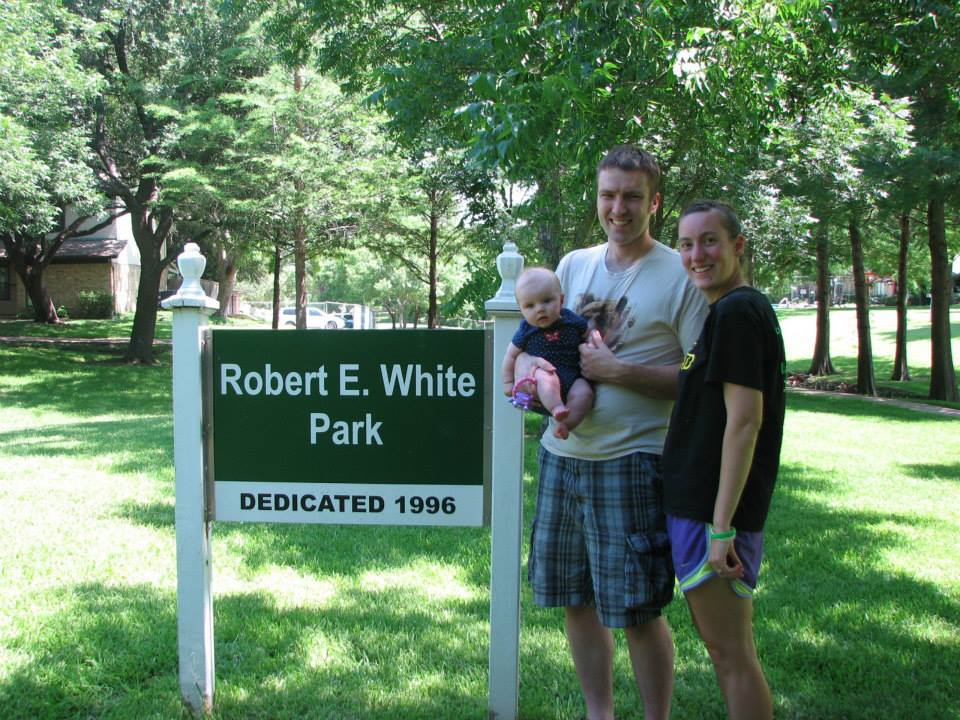
\includegraphics[angle=0]{plots/park.ps}}
 \caption{From left to right: Miss Maggie, Daryl, and Liz visiting the park
in Dallas named after Liz's grandfather. Many mosquitos as well.}
\end{figurehere}

\section{Baby Number Two}

Late this year (Table 1), we discovered that Liz was pregnant.
While this was not by design, we were, nonetheless, very happy for the news.
The Christmas card picture included in the supplementary materials depicts
how we shared the news with Daryl's side of the family.  They were tasked
with taking our picture and we unfurled the shown banner in front of them.
Air temperatures were below 0\degC at the time, so the shared moment did 
not last long!  Also, behind Daryl is a small tree planted by Grandma
Barb to commerate Miss Maggie's birth. The other trees in the background 
were planned close to Daryl's birth.

Planning is well underway to accomodate this newest child.  We have not
fully resolved how the sleeping arrangements will work, but we suspect 
Miss Maggie will remain in her crib for a while yet while the newborn 
will sleep in a smaller crib.  We plan to continue the use of cloth 
diapers with the next child and Daryl hopes for another girl for the purposes
of reusing all of Miss Maggie's stuff!  

\section{Summary}

This year has been the best on record for our growing family.  We expect
things to continue to get better with the passing years.

\bigskip
  \emph{Acknowledgments} Our family wishes to thank you for the generous 
support, prayers, cards, gifts, and visits you have provided us in the past
year. With your continued support, this letter will be produced again
next year. Please note that the format choosen for this correspondance was
completely Daryl's idea and doing. Full \LaTeX\xspace source can be found on 
Daryl's github page.

\section{References}

\refer Github, 2013: https://github.com/akrherz/me , visited 7 Dec 2013.
\refer King David, ~700 BC: Psalm 127: 3-5 \vol 1.

\end{multicols}

\end{document}

